%Chap 4a pag 24
\definecolor{Purple}{RGB}{153,0,153}
\definecolor{Green}{RGB}{0,100,0}

\begin{frame}{Optimalidad de A* (más útil)}
\textcolor{Green}{Lema:} A* expande los nodos en orden creciente de valor
\textcolor{Purple}{$f$}.\\[0.2 cm]
Agrega gradualmente "\textcolor{Purple}{$f$}-contornos" de nodos (Agregar capas en
amplitud).\\
Contorno \textcolor{Purple}{i} tiene todos los nodos con \textcolor{Purple}{$f=f_i$},
cuando \textcolor{Purple}{$f_i < f_{i+1}$}
\begin{figure}
    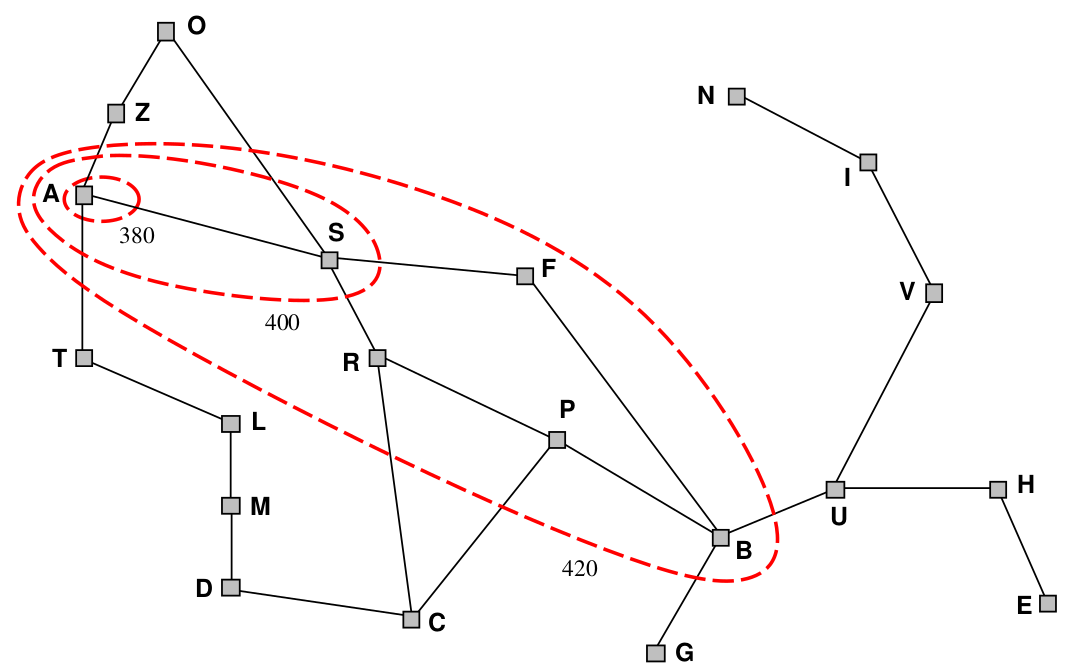
\includegraphics[scale=0.2]{24_chap4a_pag24.png}
\end{figure}
\end{frame}{}
